\section{Problem Description}
\label{sec:description}

We begin to set the problem up in this section, beginning with the geometry of
the sensor and the three-phase power lines. We assume that the world $y$-axis
coincides with the axial direction of the power lines.
Figure~\ref{fig:geometry}, therefore, shows the power lines in the
$q=(x,z)$-plane.
%
\begin{figure}[tbh]
  \centering
  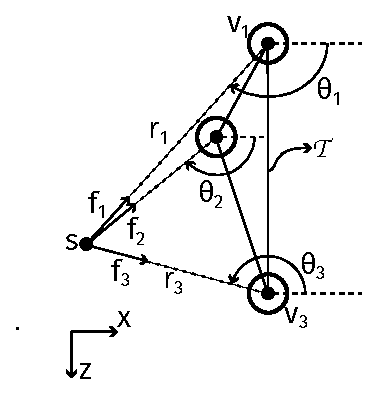
\includegraphics[width=0.35\textwidth]{./figures/general_power_line.eps}
  \caption{Arbitrary power line geometry: $r_\alpha = \nicefrac{\xi}{e_\alpha}$
  is the distance from power line $v_\alpha$ to the sensor $s$. $\theta_\alpha$
is the angle the unit vector $-f_\alpha$ from $v_\alpha$ to $s$ makes with the
world's $x$-axis. $\mc{T}$ is the triangle formed by the three wires.}
  \label{fig:geometry}
\end{figure}
%
The sensor is depicted by $s$ in this figure, and has the coordinates $(x, z)$
in the plane. Each power line is depicted by $\{v_\alpha\}_{i=1}^3$ and its
coordinates in the world frame is given by $(x_\alpha, z_\alpha)$. The distance
from the wire $v_\alpha$ to the sensor $s$ is $r_\alpha$ and is inversely
proportional to the peak electric field magnitude $e_\alpha$ generated by that
wire. From Section~\ref{sec:em_field}, we know that this constant is given by
%
\begin{equation}
    r_\alpha = \frac{\xi}{e_\alpha} = \frac{\alpha c \mu_0
I_0}{2\pi}\frac{1}{e_\alpha}.
\label{eq:xi_defn}
\end{equation}
%
The angle $\theta_\alpha$ is defined to be between the world's $x$-axis and the
vector opposite to the unit vector, $f_\alpha$, that points from the sensor $s$
to the wire $v_\alpha$. The triangle formed by the three wires is named
$\mc{T}$.

With this set-up, our problem is to devise an estimation/control strategy that
utilizes the rms electric or magnetic field that will take a fully-actuated UAV
from an arbitrary point in the $(x,z)$-space to one of the power wires in order
to install a sensor. Note that, we assume that we are able to align the UAV's
body $y$-axis axially with the wire. This may be achieved by having an
independent control system that regulates the yaw rotation such that the UAV's
body $y$-axis aligns with the unit vector along the Poynting vector~\cite{},
$\bm{P}$ computed using $\bm{P} = \nicefrac{1}{\mu_0}\bm{E} \times \bm{B}$.
